\documentclass[12pt,]{article}
\usepackage{lmodern}
\usepackage{amssymb,amsmath}
\usepackage{ifxetex,ifluatex}
\usepackage{fixltx2e} % provides \textsubscript
\ifnum 0\ifxetex 1\fi\ifluatex 1\fi=0 % if pdftex
  \usepackage[T1]{fontenc}
  \usepackage[utf8]{inputenc}
\else % if luatex or xelatex
  \ifxetex
    \usepackage{mathspec}
  \else
    \usepackage{fontspec}
  \fi
  \defaultfontfeatures{Ligatures=TeX,Scale=MatchLowercase}
\fi
% use upquote if available, for straight quotes in verbatim environments
\IfFileExists{upquote.sty}{\usepackage{upquote}}{}
% use microtype if available
\IfFileExists{microtype.sty}{%
\usepackage{microtype}
\UseMicrotypeSet[protrusion]{basicmath} % disable protrusion for tt fonts
}{}
\usepackage[margin=1in]{geometry}
\usepackage{hyperref}
\hypersetup{unicode=true,
            pdftitle={Chapter 2 Draft},
            pdfborder={0 0 0},
            breaklinks=true}
\urlstyle{same}  % don't use monospace font for urls
\usepackage{graphicx,grffile}
\makeatletter
\def\maxwidth{\ifdim\Gin@nat@width>\linewidth\linewidth\else\Gin@nat@width\fi}
\def\maxheight{\ifdim\Gin@nat@height>\textheight\textheight\else\Gin@nat@height\fi}
\makeatother
% Scale images if necessary, so that they will not overflow the page
% margins by default, and it is still possible to overwrite the defaults
% using explicit options in \includegraphics[width, height, ...]{}
\setkeys{Gin}{width=\maxwidth,height=\maxheight,keepaspectratio}
\IfFileExists{parskip.sty}{%
\usepackage{parskip}
}{% else
\setlength{\parindent}{0pt}
\setlength{\parskip}{6pt plus 2pt minus 1pt}
}
\setlength{\emergencystretch}{3em}  % prevent overfull lines
\providecommand{\tightlist}{%
  \setlength{\itemsep}{0pt}\setlength{\parskip}{0pt}}
\setcounter{secnumdepth}{0}
% Redefines (sub)paragraphs to behave more like sections
\ifx\paragraph\undefined\else
\let\oldparagraph\paragraph
\renewcommand{\paragraph}[1]{\oldparagraph{#1}\mbox{}}
\fi
\ifx\subparagraph\undefined\else
\let\oldsubparagraph\subparagraph
\renewcommand{\subparagraph}[1]{\oldsubparagraph{#1}\mbox{}}
\fi

%%% Use protect on footnotes to avoid problems with footnotes in titles
\let\rmarkdownfootnote\footnote%
\def\footnote{\protect\rmarkdownfootnote}

%%% Change title format to be more compact
\usepackage{titling}

% Create subtitle command for use in maketitle
\providecommand{\subtitle}[1]{
  \posttitle{
    \begin{center}\large#1\end{center}
    }
}

\setlength{\droptitle}{-2em}

  \title{Chapter 2 Draft}
    \pretitle{\vspace{\droptitle}\centering\huge}
  \posttitle{\par}
    \author{}
    \preauthor{}\postauthor{}
    \date{}
    \predate{}\postdate{}
  
\usepackage{booktabs}
\usepackage{longtable}
\usepackage{array}
\usepackage{multirow}
\usepackage{wrapfig}
\usepackage{float}
\usepackage{colortbl}
\usepackage{pdflscape}
\usepackage{tabu}
\usepackage{threeparttable}
\usepackage{threeparttablex}
\usepackage[normalem]{ulem}
\usepackage{makecell}
\usepackage{xcolor}

\usepackage{setspace}\doublespacing

\begin{document}
\maketitle

Here I'm going to try to understand our data a bit better and state our
hypothesis.

First I start with an abstract that could be our guide for hypothesis
testing and analyses.

\#Abstract (draft)

Plant pollinator interactions are a keystone process for ecosystem
functioning. However, we lack comprehensive information from both plants
and pollinators that can inform from this mutualistic interaction
worldwide. In order to tackle this, we have selected 30 networks
distributed across the world and looked for key floral traits of
plant-pollinator interactions for a total of 1600 species. Here we look
how these floral traits shape the different plant-pollinator networks
and the main fuctional groups of insect pollinating species. Giving the
different nature of the data collated we do not compare across networks
and we focus on the main general patterns/results within network. We
have conducted our analysis at 3 levels, 1) unique networks, 2) metawebs
and by 3) grouping both. We find that specific traits are associated
with different guilds of floral visitors within these networks. We also
highlight the lack of information about traits and the reproductive
biology of the plant species of these networks. Our work shows the
importance of deepen in species traits in order to understand key
processes that can be seen with network metrics and highlights the
importance of elemental ecology for species conservation.

\emph{What sort of data do we have?}

There are approximately 1600 species from 30 different networks. All of
these networks are phytocentric (built from plants). The different
plant-pollinator communities have been studied with very different
sampling effort and methodologies. Therefore, our aim is not to compare
across studies but to create a general picture of how floral traits
shape the different pollinator taxa and network metrics. Here, we
combine the studies with multiple years of sampling and multiple sites
within an area in metawebs. These networks give a broader perspective of
the sampling area and inform about the regional species pool (Noreika et
al. 2019). The data of these networks is quantitative (visitation) or
qualitative (binary), there are in total 19 and 11 networks/metawebs of
each, respectively.

\begin{landscape}

\begingroup\fontsize{7}{9}\selectfont

\begin{longtabu} to \linewidth {>{\raggedright}X>{\raggedright}X>{\raggedright}X>{\raggedright}X>{\raggedright}X>{\raggedright}X>{\raggedleft}X>{\raggedleft}X>{\raggedleft}X>{\raggedright}X>{\raggedright}X>{\raggedright}X}
\toprule
Id & Longitude & Latitude & Country & Year & Networks & Plant spp & Pollinator spp & Network size & Sampling method & Sampling & Data type\\
\midrule
\endfirsthead
\multicolumn{12}{@{}l}{\textit{(continued)}}\\
\toprule
Id & Longitude & Latitude & Country & Year & Networks & Plant spp & Pollinator spp & Network size & Sampling method & Sampling & Data type\\
\midrule
\endhead
\
\endfoot
\bottomrule
\endlastfoot
\rowcolor{gray!6}  Bartomeus 2008 & 3.296797 & 42.315336 & Spain & 2005 & 3 & 18 & 37 & 666 & Plots with transects & Phytocentric & Quantitative\\
\addlinespace
Fang 2012 & 99.63806 & 27.90139 & China & 2008-2010 & 3 & 130 & 247 & 32110 & Plots & Phytocentric & Quantitative\\
\addlinespace
\rowcolor{gray!6}  Inouye 1990 & 135.866667 & 35.166667 & Japan & 1984-1987 & 4 & 114 & 883 & 100662 & Transects & Phytocentric & Quantitative\\
\addlinespace
Inouye 1988 & 148.266667 & -36.45 & Australia & 1983-1984 & 1 & 40 & 85 & 3400 & Plots & Phytocentric & Quantitative\\
\addlinespace
\rowcolor{gray!6}  Kaiser-Bunbury 2009 & 57.443254 & -20.452076 & Republic of Mauritius & 2003-2004 & 2 & 96 & 184 & 17664 & Plots & Phytocentric & Quantitative\\
\addlinespace
Kaiser-Bunbury 2014 & 55.43333 & -4.666667 & Republic of Seychelles & 2007-2008 & 6 & 37 & 341 & 12617 & Transects & Phytocentric & Quantitative\\
\addlinespace
\rowcolor{gray!6}  Kato 2000 & 129.493741 & 28.377248 & Japan & 1996-1999 & 16 & 110 & 609 & 66990 & Transects & Phytocentric & Quantitative\\
\addlinespace
Kevan 1970 & -71.3 & 81.816667 & Canada & 1967 & 1 & 20 & 91 & 1820 & Randow census walks & Phytocentric & Qualitative\\
\addlinespace
\rowcolor{gray!6}  Lundgren 2005 & -52 & 71 & Greenland & 2002 & 1 & 17 & 26 & 442 & Randow census walks & Phytocentric & Quantitative\\
\addlinespace
Olesen 2002 1 & 57.43 & -20.25 & Republic of Mauritius & 1998-1999 & 1 & 17 & 26 & 442 & Plots & Phytocentric & Quantitative\\
\addlinespace
\rowcolor{gray!6}  Mcmullen 1993 & -90.600747 & -0.290164 & Ecuador & NA & All islands & 105 & 54 & 5670 & - & Phytocentric & Qualitative\\
\addlinespace
Bartomeus 2008 & 3.296797 & 42.315336 & Spain & 2005 & 3 & 13 & 37 & 481 & Plots with transects & Phytocentric & Quantitative\\
\addlinespace
\rowcolor{gray!6}  Primack 1983 1 & 171.566667 & -42.95 & New Zealand & 1976-1978 & 1 & 18 & 60 & 1080 & Randow census walks & Phytocentric & Qualitative\\
\addlinespace
Primack 1983 2 & 171.78466 & -43.02823 & New Zealand & 1976-1978 & 1 & 41 & 139 & 5699 & Randow census walks & Phytocentric & Qualitative\\
\addlinespace
\rowcolor{gray!6}  Primack 1983 3 & 171.720224 & -43.099531 & New Zealand & 1976-1978 & 1 & 49 & 118 & 5782 & Randow census walks & Phytocentric & Qualitative\\
\addlinespace
Ramirez 1989 & -61.716667 & 5.583333 & Venezuela & NA & 1 & 48 & 49 & 2352 & Randow census walks & Phytocentric & Qualitative\\
\addlinespace
\rowcolor{gray!6}  Ramirez 1992 & -67.416667 & 8.933333 & Venezuela & 1983,1984,1989 & 1 & 28 & 53 & 1484 & Randow census walks & Phytocentric & Qualitative\\
\addlinespace
Robertson 1929 & -89.8968771 & 39.278958 & United States & 1997-1899 & NA & 456 & 1044 & 476064 & - & Phytocentric & Qualitative\\
\addlinespace
\rowcolor{gray!6}  Small 1976 & -75.5 & 45.4 & Canada & 1973 & 1 & 13 & 34 & 442 & 10h per spp & Phytocentric & Quantitative\\
\addlinespace
Souza 2018 & -57.885 & -21.701111 & Brazil & 2008-2009 & 1 & 62 & 89 & 5518 & Plots & Phytocentric & Quantitative\\
\addlinespace
\rowcolor{gray!6}  Traveset 2013 & -91.012863 & -0.6907 & Ecuador & 2010-2011 & 1 & 60 & 220 & 13200 & Randow census walks & Phytocentric & Quantitative\\
\addlinespace
Bartomeus 2015 unp. & -6.16895 & 37.234966 & Spain & 2015 & 16 & 57 & 277 & 15789 & Transects & Phytocentric & Quantitative\\
\addlinespace
\rowcolor{gray!6}  Bek 2006 & 10.216667 & 56.066667 & Denmark & 2003 & 1 & 37 & 225 & 8325 & Plots & Phytocentric & Qualitative\\
\addlinespace
Olesen 2002 2 & -31 & 39.4 & Azores & 2000 & 1 & 10 & 12 & 120 & Plots & Phytocentric & Quantitative\\
\addlinespace
\rowcolor{gray!6}  Bundgaard 2003 & 10.233333 & 56.066667 & Denmark & 2003 & 1 & 16 & 44 & 704 & Plots & Phytocentric & Qualitative\\
\addlinespace
Chacoff 2011 & -68.015892 & -32.008985 & Argentina & 2006-2009 & 4 & 59 & 196 & 11564 & Plots & Phytocentric & Quantitative\\
\addlinespace
\rowcolor{gray!6}  Dicks 2002 & 1.575532 & 52.762395 & England & 2001? & 2 & 23 & 80 & 1840 & Plots & Phytocentric & Quantitative\\
\addlinespace
Dupont 2009 & 9.1 & 6.1 & Denmark & 2005 & 2 & 31 & 329 & 10199 & Plots & Phytocentric & Quantitative\\
\addlinespace
\rowcolor{gray!6}  Elberling 1999 & 18.5 & 68.35 & Sweden & 1994 & 1 & 24 & 118 & 2832 & Plots with transects & Phytocentric & Quantitative\\
\addlinespace
Dupont 2009 2 & -20.5 & 74.5 & Greenland & 1996-1997 & 1 & 31 & 76 & 2356 & Random census walks & Phytocentric & Qualitative\\*
\end{longtabu}
\endgroup{}
\end{landscape}

\newpage

\textbf{PLOT 1}

Here I show the percentage or orders from the different species without
consider visitation and just richness of species. Therfore, if we have a
network with 4 species from from different orders, each will appear as
25\% within the stack bar of the barplot.

\vspace{4cm}

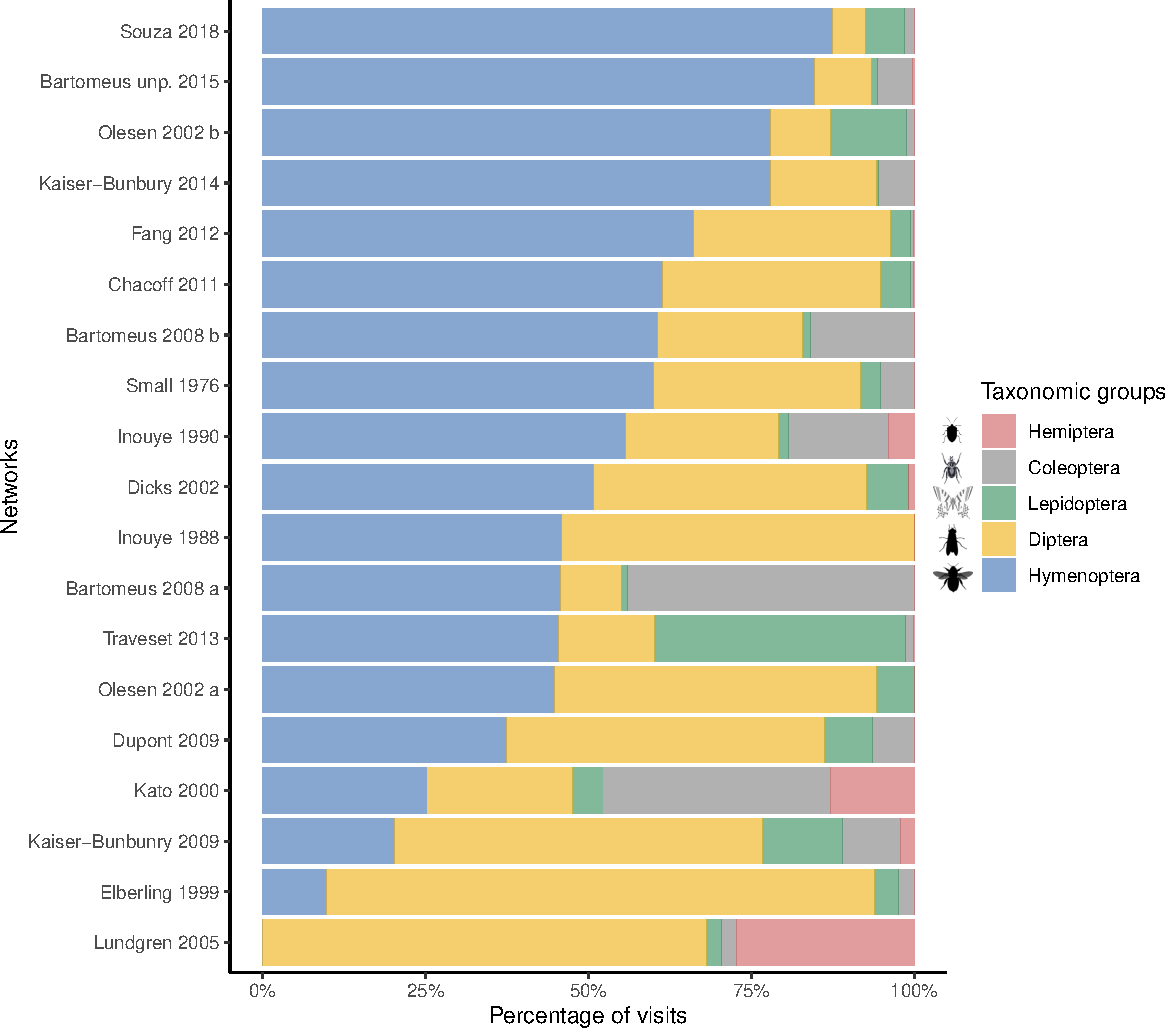
\includegraphics{Draft_files/figure-latex/unnamed-chunk-2-1.pdf}

\newpage

\vspace{4cm}

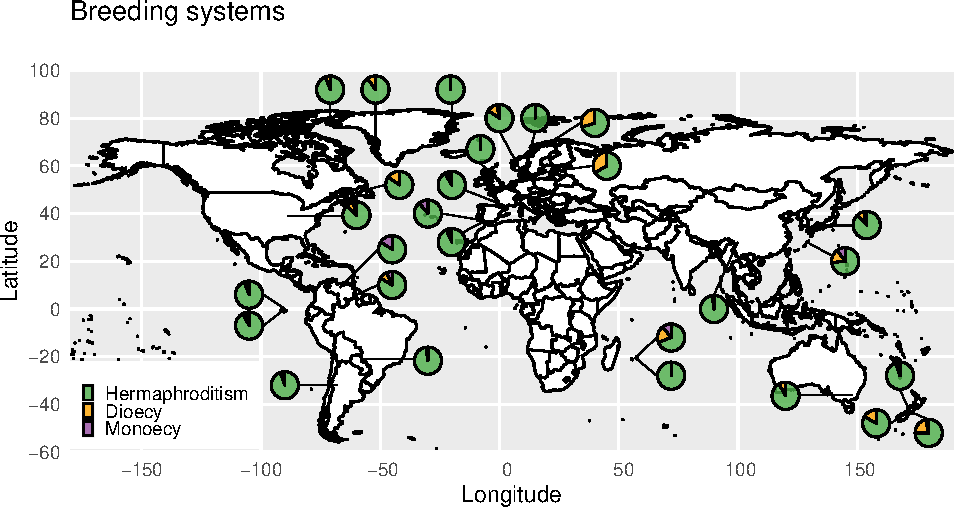
\includegraphics{Draft_files/figure-latex/unnamed-chunk-3-1.pdf}

\newpage

\textbf{PLOT 2}

\begin{center}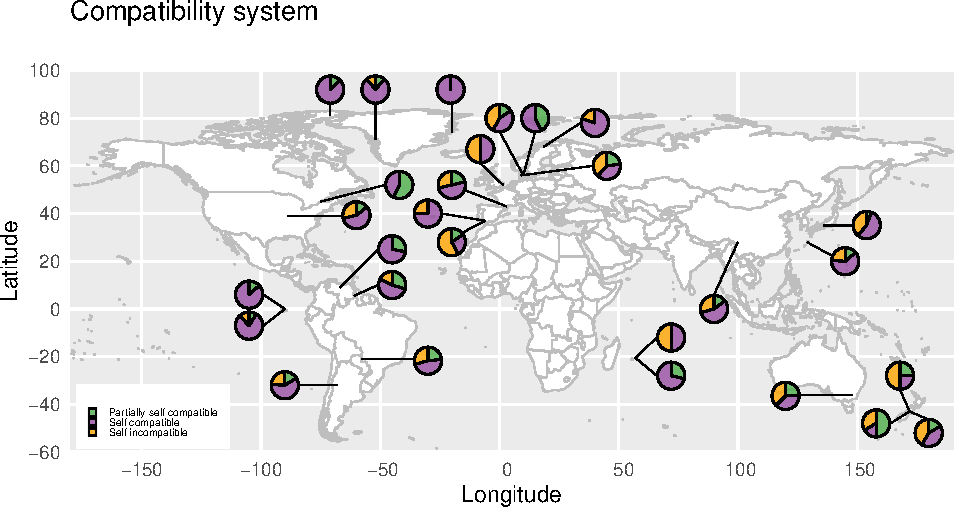
\includegraphics{Draft_files/figure-latex/unnamed-chunk-4-1} \end{center}

\newpage

\textbf{PLOT 3}

\begin{center}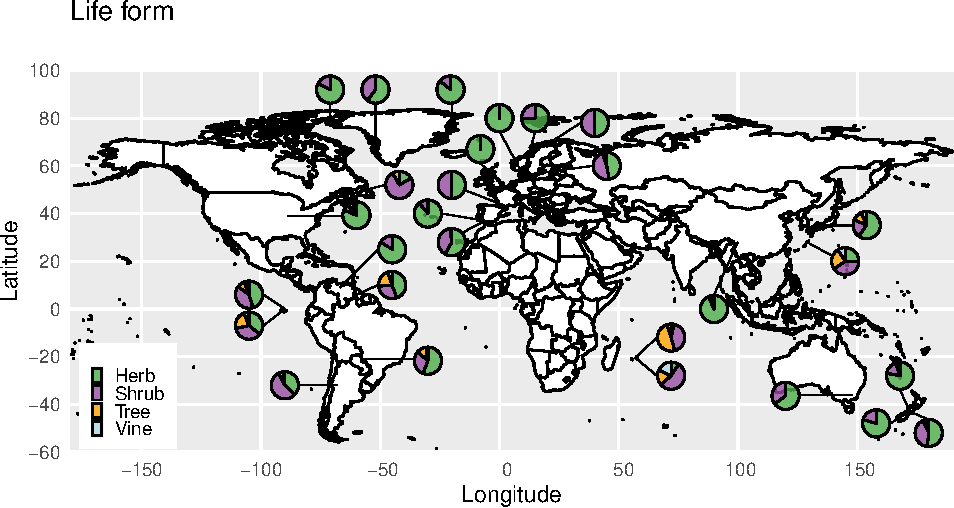
\includegraphics{Draft_files/figure-latex/unnamed-chunk-5-1} \end{center}

\newpage

\textbf{PLOT 4}

\begin{center}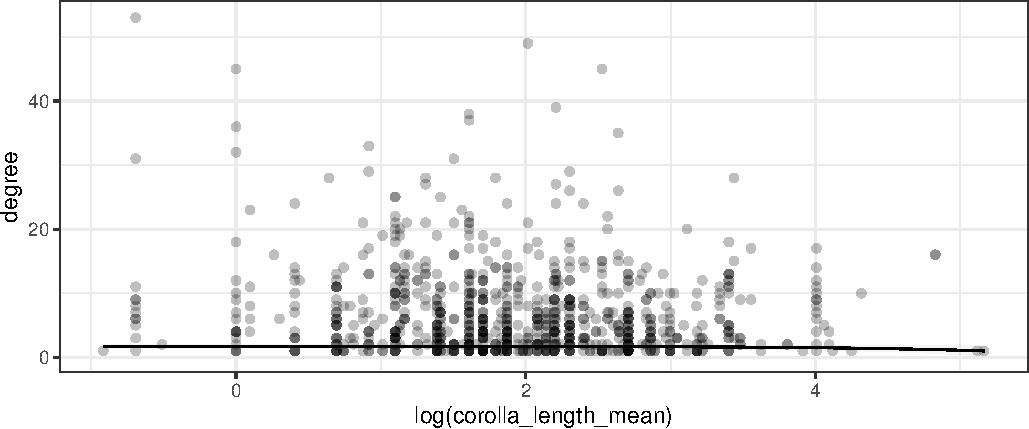
\includegraphics{Draft_files/figure-latex/unnamed-chunk-6-1} \end{center}

\#REFERENCES

\hypertarget{refs}{}
\leavevmode\hypertarget{ref-noreika2019pollinator}{}%
Noreika, Norbertas, Ignasi Bartomeus, Marie Winsa, Riccardo Bommarco,
and Erik Öckinger. 2019. ``Pollinator Foraging Flexibility Mediates
Rapid Plant-Pollinator Network Restoration in Semi-Natural Grasslands.''
\emph{Scientific Reports} 9 (1). Nature Publishing Group: 1--11.


\end{document}
